%% silkpage_coat_of_arms_06.tex — Lotus and Stronger Eastern Recursion
%%
%% Uses:
%% - Lotus_10.svg as repeated heraldic charge
%% - Eastern_Pattern.svg.png as textile mantle reference and embedded pattern field
%% - Y combinator verbatim
%% - lambda as generative stem
%% - Boteh Jeghe as Persian charge
%%
%% compile: xelatex silkpage_coat_of_arms_06.tex

\documentclass[border=24pt]{standalone}
\usepackage{tikz}
\usepackage{fontspec}
\usepackage{xcolor}
\usepackage{graphicx}
\usetikzlibrary{calc}

\newfontfamily\latinfont[
  Path=/System/Library/Fonts/,
  Ligatures=TeX, Kerning=On, Numbers=OldStyle
]{SFNS.ttf}

\definecolor{silkgreen}{HTML}{566E41}
\definecolor{deepgreen}{HTML}{26630A}
\definecolor{sage}{HTML}{DCE5D4}
\definecolor{maroon}{HTML}{57160F}
\definecolor{orange}{HTML}{E97E00}
\definecolor{paper}{HTML}{FFFFFF}
\definecolor{lightgray}{HTML}{DDDDDD}
\definecolor{ink}{HTML}{333333}

\pagecolor{paper}

\newcommand{\lotusglyph}[3]{%
  \node[inner sep=0pt] at (#1,#2) {
\includegraphics[width=#3]{Lotus_10.svg.png}};
}

\newcommand{\boteh}[4]{%
  \begin{scope}[shift={(#1,#2)}, scale=#3]
    \path[fill=#4, draw=none]
      (0,0)
        .. controls (0.85,0.08) and (1.28,0.85) .. (1.2,1.82)
        .. controls (1.08,3.18) and (0.38,4.36) .. (-0.26,5.06)
        .. controls (-0.86,5.74) and (-1.42,5.68) .. (-1.76,5.1)
        .. controls (-2.02,4.64) and (-1.94,4.1) .. (-1.56,3.74)
        .. controls (-1.12,3.34) and (-0.68,3.3) .. (-0.12,3.66)
        .. controls (0.12,2.86) and (0.12,2.06) .. (-0.04,1.18)
        .. controls (-0.22,0.28) and (-0.54,-0.2) .. (-1.06,-0.86)
        .. controls (-0.62,-0.34) and (-0.22,-0.02) .. (0,0)
      -- cycle;
    \path[fill=paper, draw=none, opacity=0.93]
      (-0.18,0.48)
        .. controls (0.4,0.9) and (0.62,1.62) .. (0.56,2.36)
        .. controls (0.48,3.24) and (0.02,4.0) .. (-0.46,4.52)
        .. controls (-0.78,4.86) and (-1.04,4.88) .. (-1.2,4.58)
        .. controls (-1.34,4.3) and (-1.24,3.98) .. (-0.96,3.76)
        .. controls (-0.68,3.54) and (-0.44,3.52) .. (-0.14,3.68)
        .. controls (0.02,3.1) and (0.06,2.4) .. (-0.08,1.64)
        .. controls (-0.16,1.2) and (-0.3,0.84) .. (-0.48,0.5)
      -- cycle;
  \end{scope}
}

\newcommand{\recursivebotehchain}[5]{%
  \foreach \dx/\dy/\sc/\op in {0/0/1/0.95,0.62/0.56/0.72/0.82,1.04/0.98/0.5/0.68,1.34/1.34/0.34/0.54} {%
    \begin{scope}[shift={(#1,#2)}, rotate=#4]
      \begin{scope}[shift={(\dx,\dy)}, scale=#3]
        \fill[#5, opacity=\op] (0,0) circle (0.045);
        \boteh{0}{0}{\sc}{#5}
      \end{scope}
    \end{scope}
  }%
}

\begin{document}
\begin{tikzpicture}[x=1cm,y=1cm,line cap=round,line join=round]

  %% background textile mantle using eastern pattern
  \node[opacity=0.12, rotate=6] at (-4.7,4.9) {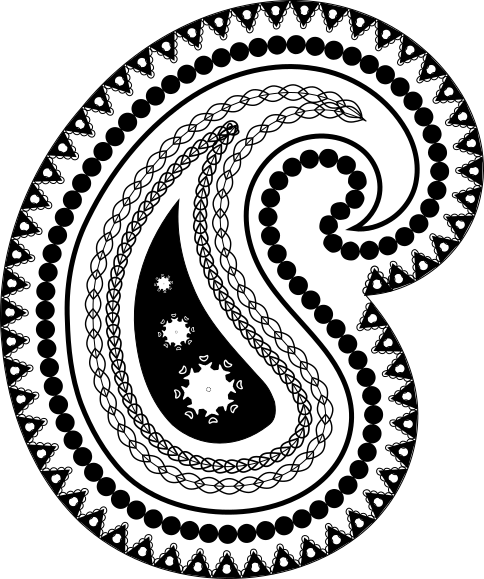
\includegraphics[width=7.5cm]{Eastern_Pattern.svg.png}};
  \node[opacity=0.12, rotate=-6, xscale=-1] at (4.7,4.9) {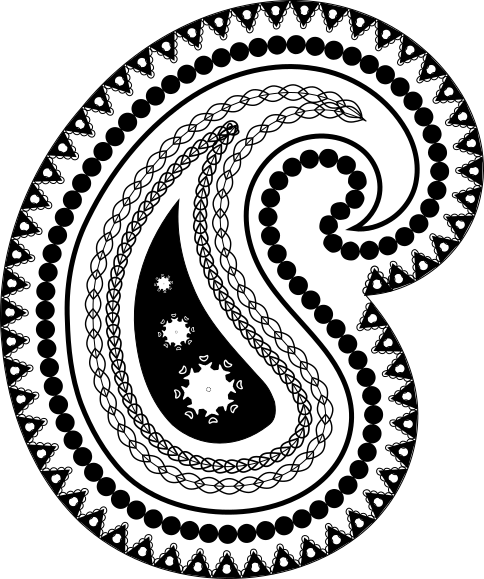
\includegraphics[width=7.5cm]{Eastern_Pattern.svg.png}};
  \node[opacity=0.06, rotate=90] at (0,1.6) {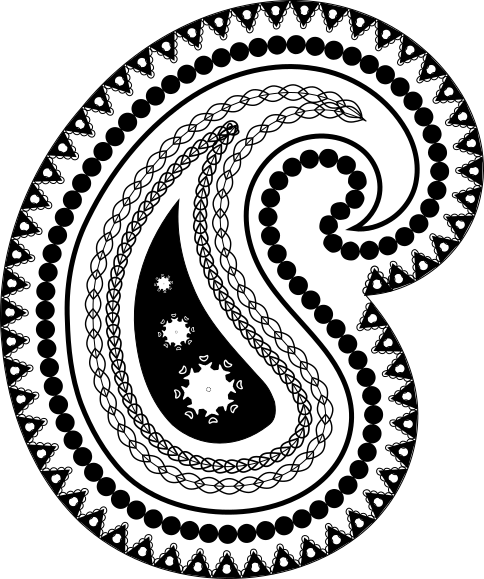
\includegraphics[width=7.4cm]{Eastern_Pattern.svg.png}};

  %% title
  \node[font=\latinfont\fontsize{38pt}{40pt}\selectfont, text=silkgreen] at (0,13.35) {SilkPage};
  \node[font=\latinfont\fontsize{10pt}{12pt}\selectfont, text=ink] at (0,12.64)
    {lotus, lambda, boteh, and eastern recursive textile structure};

  %% top wave
  \draw[silkgreen, line width=0.95pt, samples=220, smooth, domain=-7.0:7.0]
    plot(\x, {10.82 + 0.12*sin(58*\x)});
  \draw[orange, line width=0.7pt, samples=220, smooth, domain=-7.0:7.0]
    plot(\x, {10.63 + 0.1*sin(58*\x + 20)});
  \foreach \x in {-6.0,-4.7,-3.4,-2.1,-0.8,0.8,2.1,3.4,4.7,6.0} {
    \fill[orange] (\x,{10.82 + 0.12*sin(58*\x)}) circle (0.04);
  }

  %% central lotus crest on lambda stem
  \draw[orange, line width=0.88pt] (0,12.0) -- (0,11.24);
  \draw[silkgreen, line width=0.95pt] (0,11.24) -- (-0.34,10.72) -- (-0.1,10.72);
  \draw[silkgreen, line width=0.95pt] (0,11.24) -- (0.34,10.72) -- (0.1,10.72);
  \lotusglyph{0}{12.06}{0.64cm}

  %% side standards with lotus
  \draw[orange, line width=0.88pt] (-5.92,8.72) -- (-6.36,1.18);
  \draw[orange, line width=0.88pt] (5.92,8.72) -- (6.36,1.18);
  \fill[silkgreen] (-6.08,8.29) -- (-4.93,8.29) -- (-4.72,6.74) -- (-5.89,6.74) -- cycle;
  \fill[maroon] (6.08,8.29) -- (4.93,8.29) -- (4.72,6.74) -- (5.89,6.74) -- cycle;
  \draw[orange, line width=0.68pt] (-6.08,8.29) -- (-4.93,8.29) -- (-4.72,6.74) -- (-5.89,6.74) -- cycle;
  \draw[orange, line width=0.68pt] (6.08,8.29) -- (4.93,8.29) -- (4.72,6.74) -- (5.89,6.74) -- cycle;
  \lotusglyph{-5.42}{7.49}{0.55cm}
  \lotusglyph{5.42}{7.49}{0.55cm}

  %% textile-like support vectors
  \draw[silkgreen, line width=1.02pt]
    (-6.02,10.05) .. controls (-6.72,8.95) and (-6.78,7.5) .. (-6.28,6.14)
                  .. controls (-5.92,5.1) and (-5.74,4.05) .. (-6.0,2.72)
                  .. controls (-6.22,1.68) and (-6.12,0.8) .. (-5.58,-0.1);
  \draw[silkgreen, line width=1.02pt]
    (6.02,10.05) .. controls (6.72,8.95) and (6.78,7.5) .. (6.28,6.14)
                 .. controls (5.92,5.1) and (5.74,4.05) .. (6.0,2.72)
                 .. controls (6.22,1.68) and (6.12,0.8) .. (5.58,-0.1);
  \draw[orange, line width=0.72pt, opacity=0.92]
    (-5.64,9.22) .. controls (-6.08,8.25) and (-6.03,7.18) .. (-5.74,5.92)
                 .. controls (-5.52,4.88) and (-5.44,3.78) .. (-5.62,2.28);
  \draw[orange, line width=0.72pt, opacity=0.92]
    (5.64,9.22) .. controls (6.08,8.25) and (6.03,7.18) .. (5.74,5.92)
                .. controls (5.52,4.88) and (5.44,3.78) .. (5.62,2.28);

  %% eastern recursive side chains
  \recursivebotehchain{-6.2}{0.55}{0.56}{-77}{sage!65!orange}
  \recursivebotehchain{6.2}{0.55}{0.56}{77}{sage!45!silkgreen}
  \recursivebotehchain{-5.58}{2.18}{0.42}{-67}{lightgray}
  \recursivebotehchain{5.58}{2.18}{0.42}{67}{lightgray}

  %% orbital border with repeated lotus charges
  \draw[orange!75!silkgreen, line width=0.78pt, opacity=0.72] (0,4.92) circle (3.5);
  \foreach \a in {0,15,...,345} {
    \fill[sage!72!silkgreen] (\a:3.5) circle (0.042);
  }
  \foreach \a in {90,126,162,198,234,270,306,342,18,54} {
    \begin{scope}[shift={(\a:3.5)}]
      \node[inner sep=0pt, opacity=0.95] {
\includegraphics[width=0.26cm]{Lotus_10.svg.png}};
    \end{scope}
  }
  \foreach \a in {102,138,174,210,246,282,318,354,30,66} {
    \begin{scope}[shift={(\a:4.06)}, rotate=\a-90]
      \boteh{0}{0}{0.09}{sage!78!orange}
    \end{scope}
  }

  %% shield
  \path[fill=paper, draw=silkgreen, line width=1.42pt]
    (-4.16,7.42)
      .. controls (-4.2,4.16) and (-3.72,1.74) ..
    (-2.26,-0.56)
      .. controls (-1.34,-1.78) and (-0.42,-2.66) ..
    (0,-3.02)
      .. controls (0.42,-2.66) and (1.34,-1.78) ..
    (2.26,-0.56)
      .. controls (3.72,1.74) and (4.2,4.16) ..
    (4.16,7.42) -- cycle;

  \begin{scope}
  \clip
    (-4.16,7.42)
      .. controls (-4.2,4.16) and (-3.72,1.74) ..
    (-2.26,-0.56)
      .. controls (-1.34,-1.78) and (-0.42,-2.66) ..
    (0,-3.02)
      .. controls (0.42,-2.66) and (1.34,-1.78) ..
    (2.26,-0.56)
      .. controls (3.72,1.74) and (4.2,4.16) ..
    (4.16,7.42) -- cycle;

  \fill[sage!18] (-4.3,2.04) rectangle (0,7.56);
  \fill[paper] (0,2.04) rectangle (4.3,7.56);
  \fill[sage!35] (-4.3,-3.2) rectangle (0,2.04);
  \fill[maroon!95] (0,-3.2) rectangle (4.3,2.04);

  \draw[lightgray, line width=0.36pt, opacity=0.8] (-4.16,2.04) -- (4.16,2.04);
  \draw[lightgray, line width=0.36pt, opacity=0.8] (0,7.42) -- (0,-3.02);

  %% upper-left: page with lambda producing lotuses
  \path[fill=paper, draw=silkgreen, line width=0.86pt]
    (-3.28,6.22) -- (-1.1,6.22) -- (-0.54,5.66) -- (-0.54,3.12)
    -- (-3.28,3.12) -- cycle;
  \draw[silkgreen, line width=0.76pt] (-1.1,6.22) -- (-1.1,5.88)
    .. controls (-1.1,5.5) and (-0.92,5.32) .. (-0.54,5.32);
  \node[font=\latinfont\fontsize{22pt}{22pt}\selectfont, text=silkgreen] at (-2.1,4.82) {λ};
  \draw[orange, line width=0.68pt]
    (-2.1,4.32) -- (-2.58,3.84)
    (-2.1,4.32) -- (-1.62,3.84);
  \lotusglyph{-2.74}{3.72}{0.27cm}
  \lotusglyph{-1.46}{3.72}{0.27cm}

  %% upper-right: boteh and lambda
  \boteh{2.22}{3.54}{0.34}{orange}
  \boteh{3.16}{4.12}{0.26}{maroon}
  \node[font=\latinfont\fontsize{18pt}{18pt}\selectfont, text=silkgreen] at (1.36,4.9) {λ};
  \draw[silkgreen, line width=0.78pt]
    (1.04,4.1) -- (1.76,4.1)
    (1.4,3.74) -- (1.4,4.46);

  %% lower-left: complex plane and temporal spiral
  \draw[silkgreen, line width=0.78pt] (-3.1,-1.6) -- (-0.82,-1.6);
  \draw[silkgreen, line width=0.78pt] (-1.96,-2.56) -- (-1.96,1.02);
  \node[font=\latinfont\fontsize{7pt}{8pt}\selectfont, text=ink, opacity=0.7] at (-1.0,-1.35) {Re};
  \node[font=\latinfont\fontsize{7pt}{8pt}\selectfont, text=ink, opacity=0.7] at (-1.66,0.78) {Im};
  \draw[orange, line width=0.95pt, samples=240, variable=\t, domain=0:560]
    plot ({-1.96 + 0.085*exp(\t/255)*cos(\t)},
          {-1.6 + 0.085*exp(\t/255)*sin(\t)});
  \fill[maroon] (-1.96,-1.6) circle (0.05);

  %% lower-right: eastern dotted recursive field
  \foreach \a in {0,20,...,240} {
    \pgfmathsetmacro{\rr}{0.38 + 0.008*\a}
    \pgfmathsetmacro{\xx}{2.15 + \rr*cos(\a)}
    \pgfmathsetmacro{\yy}{-0.12 + \rr*sin(\a)}
    \fill[sage] (\xx,\yy) circle (0.06);
  }
  \draw[paper, line width=0.78pt, samples=110, smooth, domain=1.35:3.0]
    plot(\x, {-0.18 + 0.22*sin(230*\x)});

  %% recursive eastern dots climbing the maroon field
  \foreach \r/\shiftx/\shifty in {0.2/2.2/-0.26,0.42/2.46/0.34,0.68/2.76/1.02,0.98/3.04/1.88} {
    \foreach \a in {20,55,...,290} {
      \pgfmathsetmacro{\xx}{\shiftx + \r*cos(\a)}
      \pgfmathsetmacro{\yy}{\shifty + 0.82*\r*sin(\a)}
      \fill[sage!92!paper, opacity=0.88] (\xx,\yy) circle (0.032 + 0.006*\r);
    }
  }

  %% central roundel with lotus and formula cartouche
  \fill[paper] (0,1.98) circle (1.64);
  \draw[silkgreen, line width=0.9pt] (0,1.98) circle (1.64);
  \draw[orange, line width=0.68pt, opacity=0.84, dash pattern=on 2pt off 2pt] (0,1.98) circle (1.26);
  \lotusglyph{0}{1.98}{0.78cm}

  \path[fill=paper, draw=silkgreen, line width=0.68pt]
    (-2.14,1.06) -- (2.14,1.06) -- (2.4,0.7) -- (2.14,0.34) -- (-2.14,0.34) -- (-2.4,0.7) -- cycle;
  \node[font=\latinfont\fontsize{8.7pt}{9.6pt}\selectfont, text=deepgreen] at (0,0.68)
    {Y = λf.(λx.f(xx))(λx.f(xx))};

  \end{scope}

  %% redraw shield
  \path[fill=none, draw=silkgreen, line width=1.42pt]
    (-4.16,7.42)
      .. controls (-4.2,4.16) and (-3.72,1.74) ..
    (-2.26,-0.56)
      .. controls (-1.34,-1.78) and (-0.42,-2.66) ..
    (0,-3.02)
      .. controls (0.42,-2.66) and (1.34,-1.78) ..
    (2.26,-0.56)
      .. controls (3.72,1.74) and (4.2,4.16) ..
    (4.16,7.42) -- cycle;

  %% bottom textile border
  \draw[orange!70!silkgreen, line width=0.72pt, samples=180, smooth, domain=-4.6:-2.0]
    plot(\x, {-4.12 + 0.08*sin(420*(\x+4.6)/2.6)});
  \draw[orange!70!silkgreen, line width=0.72pt, samples=180, smooth, domain=2.0:4.6]
    plot(\x, {-4.12 + 0.08*sin(420*(\x-2.0)/2.6)});
  \foreach \t in {0,14,...,180} {
    \pgfmathsetmacro{\rx}{3.18*cos(\t)}
    \pgfmathsetmacro{\ry}{-3.94 + 0.4*sin(\t)}
    \fill[orange!70!silkgreen] (\rx,\ry) circle (0.036);
  }
  \foreach \offset in {-3.86,-4.16,-4.46} {
    \draw[sage!70!orange, line width=0.42pt, samples=180, smooth, domain=-3.94:3.94]
      plot(\x, {\offset + 0.035*sin(44*(\x+4)) + 0.06*cos(22*\x)});
  }

  %% small lower lotus pair
  \lotusglyph{-3.4}{-1.7}{0.34cm}
  \lotusglyph{3.4}{-1.7}{0.34cm}

  %% motto
  \path[fill=paper, draw=silkgreen, line width=0.82pt]
    (-5.45,-4.84)
      .. controls (-3.82,-5.16) and (-1.72,-5.24) ..
    (0,-5.04)
      .. controls (1.72,-5.24) and (3.82,-5.16) ..
    (5.45,-4.84)
      .. controls (3.92,-4.54) and (1.68,-4.44) ..
    (0,-4.62)
      .. controls (-1.68,-4.44) and (-3.92,-4.54) ..
    (-5.45,-4.84) -- cycle;
  \node[font=\latinfont\fontsize{11.2pt}{12.2pt}\selectfont, text=maroon] at (0,-4.76)
    {Lotus \,•\, Recur \,•\, Weave \,•\, Return};
  \node[font=\latinfont\fontsize{8pt}{9pt}\selectfont, text=silkgreen] at (0,-5.46)
    {Y = λf.(λx.f(xx))(λx.f(xx))};
  \node[font=\latinfont\fontsize{7.7pt}{8.8pt}\selectfont, text=ink, opacity=0.78] at (0,-6.02)
    {lotus and boteh under eastern recursive textile structure};

\end{tikzpicture}
\end{document}
